\documentclass[submit]{harvardml}

% FDV: Make sure all front matter has correct years, dates, book sections, etc.
\course{CS181-S23}
\assignment{Assignment \#2}
\duedate{11:59pm EST, Feb 23th, 2023}

\usepackage[OT1]{fontenc}
\usepackage[colorlinks,citecolor=blue,urlcolor=blue]{hyperref}
\usepackage[pdftex]{graphicx}
\usepackage{subfig}
\usepackage{fullpage}
\usepackage{amsmath}
\usepackage{amssymb}
\usepackage{framed}
\usepackage{color}
\usepackage{soul}
\usepackage{todonotes}
\usepackage{listings}
\usepackage{common}
\usepackage{enumitem}
\usepackage{bm}
\usepackage{bbm}
\newcommand{\B}{\text{B}}
\newcommand{\Beta}{\text{Beta}}
\newenvironment{ans}{
  \begin{enumerate}
  \color{blue}
}{
  \end{enumerate}
  \color{black}
}

\usepackage[mmddyyyy,hhmmss]{datetime}

\definecolor{verbgray}{gray}{0.9}

\lstnewenvironment{csv}{%
  \lstset{backgroundcolor=\color{verbgray},
  frame=single,
  framerule=0pt,
  basicstyle=\ttfamily,
  columns=fullflexible}}{}

\begin{document}

\begin{center}
{\Large Homework 2: Classification and Bias-Variance Trade-offs}\\
\end{center}

\subsection*{Introduction}

This homework is about classification, bias-variance trade-offs, and uncertainty quantification. In lecture we have primarily focused on binary classifiers trained to discriminate between two classes. In multiclass classification, we
discriminate between three or more classes. 
We encourage you to read
CS181 Textbook's Chapter 3 for more information on linear
classification, gradient descent, and classification in the discriminative setting. Read Chapter 2.8 for more
information on the trade-offs between bias and variance.

The datasets that we will be working with relate to astronomical observations. The first dataset, found at \verb|data/planet-obs.csv|, contains information on whether a planet was observed (as a binary variable) at given points in time. This will be used in Problem 1. The second dataset, available at \verb|data/hr.csv|, details different kinds of stars and their measured magnitude and temperature. You will work with this data in Problem 3.
As a general note, for classification problems we imagine that we have
the input matrix $\boldX \in \reals^{n \times d}$ (or perhaps they
have been mapped to some basis $\bm{\Phi}$, without loss of
generality) with outputs now ``one-hot encoded."  This means that if
there are~$K$ output classes, rather than representing the output
label $y$ as an integer~${1,2,\ldots,K}$, we represent $\boldy$ as a
``one-hot" vector of length~$K$. A ``one-hot" vector is defined as
having every component equal to 0 except for a single component which
has value equal to 1.  For example, if there are $K = 7$ classes and a
particular data point belongs to class 3, then the target vector for
this data point would be~$\boldy = [0,0,1,0,0,0,0]$.  We will define
$C_1$ to be the one-hot vector for the 1st class, $C_2$ for the 2nd
class, etc.  Thus, in the previous example $\boldy = C_3$. If there
are $K$ total classes, then the set of possible labels is $\{C_1
\ldots C_K \} = \{C_k\}_{k=1}^K$.  Throughout the assignment we will
assume that each label $\boldy \in \{C_k\}_{k=1}^K$ unless otherwise
specified. The most common exception is the case of binary classification
($K = 2$), in which case labels are the typical integers $y \in \{0, 1\}$.

In problems 1 and 3, you may use \texttt{numpy} or \texttt{scipy}, but
not \texttt{scipy.optimize} or \texttt{sklearn}. Example code given is
in Python 3.

Please type your solutions after the corresponding problems using this
\LaTeX\ template, and start each problem on a new page.

Please submit the \textbf{writeup PDF to the Gradescope assignment `HW2'}. Remember to assign pages for each question.  \textbf{You must include your plots in your writeup PDF. } The supplemental files will only be checked in special cases, e.g. honor code issues, etc.

Please submit your \textbf{\LaTeX\ file and code files to the Gradescope assignment `HW2 - Supplemental'}. 

%%%%%%%%%%%%%%%%%%%%%%%%%%%%%%%%%%%%%%%%%%%%%
% Problem 1
%%%%%%%%%%%%%%%%%%%%%%%%%%%%%%%%%%%%%%%%%%%%%

\begin{problem}[Exploring Bias-Variance and Uncertainty]
In this problem, we will explore the bias and variance of a few different model classes when it comes to logistic regression and investigate two sources of predictive uncertainty.

We are currently managing a powerful telescope that is being used to monitor and gather measurements of some planet of interest. At certain times however, our telescope is unable to detect the planet at all. The data in \verb|data/planet-obs.csv| records the observation time in the ``Time" column and whether the planet was detected in the ``Observed" column (with the value 1 representing that it was observed). Since it is expensive to use and maintain the telescope, we would like to build a model to help us schedule and find times when we are likely to detect the planet.

\begin{enumerate}

\item First split the data into 10 mini-datasets of size $N = 30$ (i.e. dataset 1 consists of the first 30 observations, dataset 2 consists of the next 30, etc. This has already been done for you). Consider the three bases $\boldsymbol\phi_1(t) = [1, t]$, $\boldsymbol\phi_2(t) = [1,
  t, t^2]$, and $\boldsymbol\phi_3(t) = [1, t, t^2, t^3, t^4, t^5]$. For each of these bases, fit a logistic regression model using sigmoid($\boldw^\top \boldsymbol\phi(t)$) to each dataset by using gradient descent to
  minimize the negative log-likelihood.  This means you will be
  running gradient descent 10 times for each basis, once for each
  dataset.
  
  Use the given starting values of $\boldw$ and a learning rate of $\eta=0.001$, take 10,000 update
  steps for each gradient descent run, and make sure to average the
  gradient over the data points at each step. These parameters,
  while not perfect, will ensure your code runs reasonably quickly. 

\item After consulting with a domain expert, we find that the probability of observing the planet is periodic as the planet revolves around its star---we are more likely to observe the planet when it is in front of its star than when it is behind it. In fact, the expert determines that observation follows the generating process $y \sim \text{Bern}(f(t))$, where $f(t) = 0.4 \times \cos(1.1t + 1) + 0.5$ for $t \in [0, 6]$ and $y \in \{0,1\}$. Note that we, the modelers, do not usually see the true data distribution. Knowledge of the true $f(t)$ is only exposed in this problem to allow for verification of the true bias.

Use the given code to plot the true process versus your learned models. Include your plots in your solution PDF.

\textbf{In no more than 5 sentences}, explain how bias and variance reflected in the 3 types of curves on the graphs.  How do the fits of the individual and mean prediction functions change?  Keeping in mind that none of the model classes match the true generating process exactly, discuss the extent to which each of the bases approximates the true process.

\item If we were to increase the size of each dataset drawn from $N = 30$ to a larger number, how would the bias and variance change for each basis? Why might this be the case? You may experiment with generating your own data that follows the true process and plotting the results, but this is \textbf{not} necessary. \textbf{Your response should not be longer than 5 sentences}.

\item Consider the test point $t = 0.1$. Using your models trained on basis $\boldsymbol\phi_3$, report the predicted probability of observation of the \textit{first} model (the model trained on the first 30 data points). How can we interpret this probability as a measure of uncertainty? Then, compute the variance of the classification probability over your 10 models at the same point $t = 0.1$. How does this measurement capture another source of uncertainty, and how does this differ from the uncertainty represented by the classification probability?

Repeat this process (reporting the first model's classification probability and the variance over the 10 models) for the point $t = 3.2$. At which point in time would you be more confident in detecting the planet? There's no right answer---you should consider the two different types of uncertainty and their implications when translating from model output to decision making. 
\end{enumerate}
\end{problem}
 \let\cleardoublepage\clearpage
\newpage

\begin{ans}
    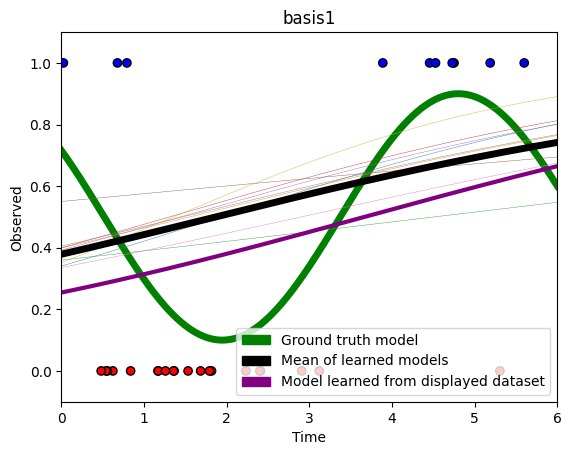
\includegraphics[scale=0.3]{hw2/basis1.png}
    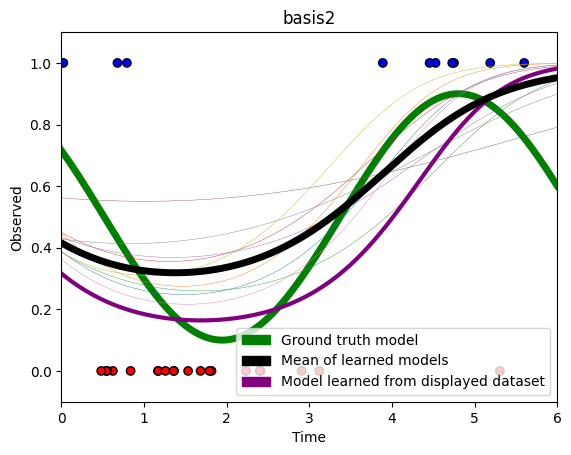
\includegraphics[scale=0.3]{hw2/basis2.png}
    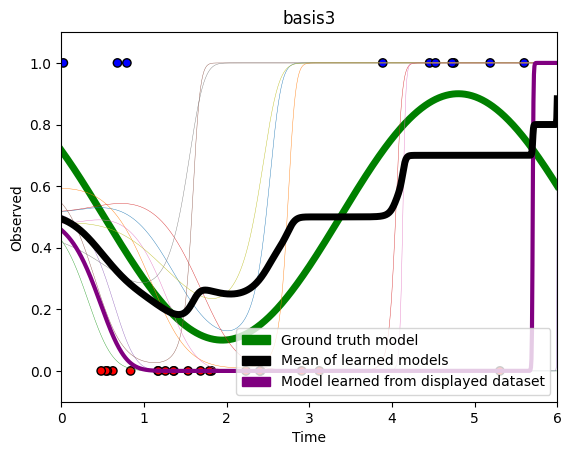
\includegraphics[scale=0.3]{hw2/basis3.png}
    \newline 
    \newline
    2. As we discussed in class, the Bias-Variance Tradeoff is that  increasing model complexity decreases error but increases the risk of overfitting and vice versa. We can see this here: for the models with bases of lower degrees, there is very high error (since the linear model cannot account for nonlinear trends), but a very low risk of overfitting (the model can hardly fit to the actual data, so, of course, it is not going to fit to the noise); conversely, for the models with high-dimensional bases, the output is more jagged than the ground-truth, so it is overfit to the noisy input data, but the variance on that input data is very low. That is, the fit to the data becomes better and better as we increase the dimensionality of our bases, but, as the dimension gets too high, the model overfits, and fits the ground-truth model worse and worse. Out of these three options, basis 3 seems to best approximate the ground truth. 
    \newline
    % ?? increasing the bias and decreasing the variance? 
    % ww defines variance as sample variance, ie mse
    % ww defines bias as how predisposed the model is to pred a value away from the ground truth
    % \item Increasing the size of the data would decrease the bias and decrease the variance
    \newline
    \item 3. Increasing the size of the training data would decrease the bias and have no effect on the variance. It would decrease the bias becuase we are minimizing loss, and, analogously, minimizing the loss at a specific point is going to be the MLE, which, since we often assume $\epsilon \sim \mathcal N(0, \sigma^2)$, implies the sample mean will be the MLE. This sample mean by LLN converges to the true value, so the bias will decrease. There will be no effect on variance because variance is more of a function of model complexity than input data. 
    \newline
    \newline
    4.
    \newline
    \qquad a) When $x = 0.1$, based on the model trained on basis 3, I got a predicted result of $0.51992796$. This implies high uncertainty because a value of $0$ means we are certain the planet can be observed and $1$ means we are certain that it cannot be observed; our value is nearly 50/50, so we are quite uncertain. The variance over our ten training sets is $0.003429945554968907$. This measure captures uncertainty from bias in the training set; however, it is relatively much lower than our uncertainty for the actual observability, implying that we are quite certain about the representativeness of our data, but much more unsure as to whether that data indicate that the planet is actually observable. 
    \newline
    \newline
    \qquad b) Repeating the process, for $\phi_3(3.1)$, I got a prediction of $\approx 0.999$ from the first model, so the first model is almost certain that the planet will be observable. However, over all ten models, I got a variance of $\approx 0.25$, which is very high. Indeed, looking at predictions, I get very small and very large values, and the mean prediction across models is $\approx 0.5$. Therefore, in a practical sense, I wouldn't be more confident in either time, but since the mean value of our predictions at $t = 0.1$ is $\approx 0.48$, but at $t = 3.2$, it was $\approx 0.5$, I will go with the latter. The high variance tells/obscures very litle in this scenario because it is variance around uncertainty in the probability. 
\end{ans}
%%%%%%%%%%%%%%%%%%%%%%%%%%%%%%%%%%%%%%%%%%%%%
% Problem 2
%%%%%%%%%%%%%%%%%%%%%%%%%%%%%%%%%%%%%%%%%%%%%

\begin{problem}[Multi-class Logistic Regression and Softmax]
The objective of this problem is to generalize binary logistic regression into the more general case of three or more classes. You will use the results of this problem to implement a classifier in Problem 3.

Consider a $K$-class model with $K \geq 3$. Suppose we have a data set $\{(\boldx_i,
\boldy_i)\}_{i=1}^n$ with features $\{\boldx_n\}_{n = 1}^N \in \mathbb{R}^d$ and one-hot encoded outputs $\{\boldy_n\}_{n = 1}^N \in \mathbb{R}^K$ (see the introduction of this homework). For a $K$-dimensional vector $\boldz = [z_1, \dots, z_K]^\top$, define the \textit{softmax} function to be
$$
\text{softmax}(\boldz) = \frac{1}{\sum_{i = 1}^K \exp(z_i)}
\begin{bmatrix}
\exp(z_1) \\
\exp(z_2) \\
\vdots \\
\exp(z_K)
\end{bmatrix}.
$$
In other words, the softmax function is a function from $\mathbb{R}^K$ to $\mathbb{R}^K$ with $k$-th component of the output
$$
\text{softmax}_k(\boldz) = \frac{\exp(z_k)}{\sum_{i = 1}^K \exp(z_i)}.
$$
We will use the shorthand notation $s_k(\boldz)$ to abbreviate the above. Note that the softmax function is the general form of the sigmoid function in binary logistic regression. This means that the derivations in this problem will be very similar to what you have seen in class.

\begin{enumerate}
  \item For $j, k \in \{1, \dots, K\}$, show that the partial derivatives of the softmax function can be written in terms of the softmax function itself in the following form:
  $$
  \frac{\partial s_k(\boldz)}{\partial z_j} = s_k(\boldz)(\delta_{jk} - s_j(\boldz))
  $$
  Here, $\delta_{jk}$ denotes the \textit{Kronecker delta} function $\delta_{jk}$:
  $$
  \delta_{jk} = 
  \begin{cases}
    1 \text{ if } j = k, \\
    0 \text{ if } j \neq k.
  \end{cases}
  $$
  Since all of these partial derivatives are with respect to scalars, you can use the typical quotient rule from your univariate calculus class. It may help to consider the cases $j = k$ and $j \neq k$ separately.
  
  Using the answer above, find the logarithmic derivatives of $\text{softmax}(\boldz)$; that is, find $\displaystyle \frac{\partial \ln s_k(\boldz)}{\partial z_j}$ for $j, k \in \{1, \dots, K\}$.
\end{enumerate}

Multi-class logistic regression has weights $\{\boldw_j\}_{j=1}^K \in \mathbb{R}^d$ for each class, which are often condensed into a single matrix $\boldW \in \mathbb{R}^{K \times d}$ (the $j$-th row of $\boldW$ corresponds to $\boldw_j$). We model the probabilities of class membership independently as
$$
p(\boldy_n = C_k | \boldx_n, \boldW) = s_k(\boldW\boldx_n)
$$
for $k \in \{1, \dots, K\}$ and $n \in \{1, \dots, N\}$.
In addition, let $y_{nk}$ denote the $k$-th component of the output vector $\boldy_n$. 
\begin{enumerate}
    \item[2.] Write out the negative log-likelihood of the data set, $\ell(\boldW) = -\ln p(\{\boldy_n\}_{n=1}^N | \{\boldx_n\}_{n=1}^N, \boldW)$, in terms of $s_k, \boldW, \{\boldx_n\}_{n=1}^N$, and $y_{nk}$. You can start by noting that for a single observation $(\boldx_n, \boldy_n)$,
    $$
    p(\boldy_n | \boldx_n, \boldW) = \prod_{k=1}^Kp(\boldy_n = C_k | \boldx_n, \boldW)^{y_{nk}}
    $$
    because $y_{nk} = 1$ if $\boldy_n$ belongs to class $C_k$ and $y_{nk} = 0$ otherwise. The equation above simply lets us combine all possible class memberships of $\boldy_i$ into a single expression. This is also known as the ``power trick" as we express the probability as a product of terms raised to a power that is either 0 or 1.
\end{enumerate}
\end{problem}

\begin{framed}
\noindent\textbf{Problem 2} (cont.)\\
\begin{enumerate}
    \item[3.] Consider the weight matrix $\boldW$ and the $i$-th feature vector $\boldx_i$. Denote their product as $\boldz_i = \boldW\boldx_i$. Compute the derivative of $\ell(\boldW)$ with respect to the $j$-th coordinate of the $K$-dimensional vector $\boldz_i$ (denoted as $z_{ij}$). In particular, show that 
    $$
    \frac{\partial \ell}{\partial z_{ij}} = \sum_{k = 1}^K y_{ik}(s_j(\boldz_i) - \delta_{kj})
    $$
    You may want to use your answer from part 1. Then, show that the above sum can be simplified:
    $$
    \sum_{k = 1}^K y_{ik}(s_j(\boldz_i) - \delta_{kj}) = s_j(\boldz_i) - y_{ij}.
    $$
    It will help to consider the case $k = j$ separately again and remove the delta function from the equation.
    \item[4.] Conclude that the gradient of negative log-likelihood with respect to a single weight vector $\boldw_j$ is given by the \textit{vector}
    $$
    \frac{\partial \ell}{\partial \boldw_j} = \sum_{n = 1}^N(s_j(\boldW\boldx_n) - y_{nj})\boldx_n
    $$
    for $j \in \{1, \dots, K\}$. This can be done by using the chain rule:
    $$
    \frac{\partial \ell}{\partial \boldw_j} = \sum_{n = 1}^N\sum_{k = 1}^K\frac{\partial \ell}{\partial z_{nk}}\frac{\partial z_{nk}}{\partial \boldw_j}.
    $$
    We found the first derivative in part 3. What do we know about the second derivative when $k \neq j$? You can start by expressing $z_{nk}$ in terms of the vectors $\{\boldw_i\}_{i=1}^K$ and $\{\boldx_i\}_{i=1}^N$.
    
    We can use this final expression to optimize the weights via gradient descent!
\end{enumerate}
\end{framed}

\newpage
\begin{ans}
    \item We can split this differentiation into two cases:
    \begin{enumerate}
        \item Case 1: $k = j$: For this case, we apply the quotient rule: 
        $$
        \frac{\partial }{\partial z_k} \frac{\exp(z_k)}{\sum_{i = 1}^K \exp(z_i)} = \frac{\exp(z_k)\sum_{i = 1}^K \exp(z_i) - \exp(2z_k)}{\left(\sum_{i = 1}^K \exp(z_i)\right)^2}
        $$
        Now, we can split the fraction into two fractions:
        $$
        \frac{\exp(z_k)\sum_{i = 1}^K \exp(z_i)}{\left(\sum_{i = 1}^K \exp(z_i)\right)^2} - \frac{\exp(2z_k)}{\left(\sum_{i = 1}^K \exp(z_i)\right)^2} = \frac{e^{z_k}}{\sum_{i = 1}^K \exp(z_i)} - \frac{e^{2z_k}}{\left(\sum_{i = 1}^K \exp(z_i)\right)^2}
        $$
        By pattern-matching, this is equal to 
        $$
        s_{k}(\mathbf z) - (s_{k}(\mathbf z))^2
        $$
        \item Case 2: $k \neq j$: we similarly apply the quotient rule
        $$
        \frac{\partial }{\partial z_j} \frac{\exp(z_k)}{\sum_{i = 1}^K \exp(z_i)} = \frac{0 \cdot \sum_{i = 1}^K \exp(z_i) - \exp(z_k)\exp(z_j)}{\left(\sum_{i = 1}^K \exp(z_i)\right)^2}
        $$
        Now we can split this expression up and get
        $$
        -\frac{\exp(z_k)}{\sum_{i = 1}^K \exp(z_i)}\frac{\exp(z_j)}{\sum_{i = 1}^K \exp(z_i)} = 0 - s_k(\mathbf z) -s_j(\mathbf z)
        $$
    \end{enumerate}
    We can simplify these two cases to the equation provided, since if 
    $k = j$, then
    $$
    s_{k}(\mathbf z) - (s_{k}(\mathbf z))^2 = \frac{\partial s_k(\boldz)}{\partial z_j} = s_k(\boldz)(\delta_{jk} - s_j(\boldz))
    $$
    (where $\delta_{jk} = 1$), and if $k \neq j$, then 
    $$
    0 - s_k(\mathbf z) -s_j(\mathbf z) = \frac{\partial s_k(\boldz)}{\partial z_j} = s_k(\boldz)(\delta_{jk} - s_j(\boldz))
    $$
    \newline
    \newline
    We can find logarithmic derivative in general as follows, from the chain rule:
    $$
    \frac{d}{dx}\ln f(x) = \frac{1}{f(x)}\frac{df(x)}{dx} = \frac{f'(x)}{f(x)}
    $$
    Thus, we can plug in:
    $$
    = \frac{s_k(\boldz)(\delta_{jk} - s_j(\boldz))}{s_k(\boldz)} = \delta_{jk} - s_j(\boldz)
    $$
    \item Since we want 
    $$
    P(\left\{\mathbf x_i, \mathbf y_i\right\}_{j = 1}^n) = \prod_{j = 1}^n\left(\prod_{k = 1}^K s_k(\mathbf{Wx_n})\right)^{\mathbf y_{jk}}
    $$
    By the Multiplication Rule. Now we take the log. To do this, we must first find the log of the sigmoid. In general, we can apply rules of logs:
    $$
    -\ln s_k(\mathbf z) = \ln(e^{\mathbf z_k}) - \ln(\sum_{j = 1}^K e^{\mathbf z_j}) =  \sum_{j = 1}^K \mathbf z_j - \mathbf z_k
    $$
    Now, applying our negative log from above, we get
    $$
    \sum_{j = 1}^n\mathbf \left(\mathbf \sum_{k = 1}^K  y_{jk} \ln(s_k(\mathbf{Wx}_j))\right)
    % = \sum_{j = 1}^n\mathbf y_{jk}\left[ \sum_{k = 1}^K \left(\sum_{j = 1}^K \mathbf z_j - \mathbf z_k\right)\right]
    $$
    \item We know that the derivative of a sum is the sum of derivatives. Therefore, we can drop all but one term from our result from part 2 and get:
    $$
    \frac{\partial}{\partial \matbf z_{ij}}\mathbf \sum_{k = 1}^K y_{jk}\ln(s_k(\mathbf{Wx}_j))
    $$
    Now, we can apply this rule again. Since we are deriving w.r.t. $z_{ij}$, $\mathbf y_{jk}$ is a constant. Thus, we only need to differentiate $\ln(s_k(\mathbf{Wx}_j))$, which we did in part 1. We can plug in for that and get 
    $$
    \frac{\partial}{\partial \matbf z_{ij}}\mathbf \sum_{k = 1}^K y_{jk}\ln(s_k(\mathbf{Wx}_j)) = \frac{\partial}{\partial \matbf z_{ij}}\mathbf \sum_{k = 1}^K y_{jk}(s_{j}(\mathbf z_i) - \delta_{kj})
    $$
    Finally, notice that we have coefficient $y_{jk}$. This reflects element in a matrix of one-hot row vectors; thus, it will be zero or one. Further, it will only be one for one class, so we can set $y_{jk}$ to one for one class, distribute, and evaluate the sum; all terms where $y_{jk} = 0$ will get dropped. From here, we analyze the cases where $k = j$ and $k \neq j$:
    \begin{enumerate}
        % \item $k = j$: then our Kronecker delta function will evaluate to 1. We only care about cases where $y_{ij}$ equals one as well. When $k = j$, There will be one such case. Therefore, we have 
        % $$
        % s_j(\boldz_i) - y_{ij}.
        % $$
        % \item $k \neq j$: then our Kronecker delta function will evaluate to 0. Furhrur function will only be nonzero when $y_{ij} = 1$ and $k = j$ because, if the first condition is false, then we drop the term, and if the second term is false, 
        % then the term becomes a constant, and we can drop it.  
        \item $k = j$ Let's write the sum where $k = j$: we have 
        $$
        \sum_{k \in \{[1, K] : k = j\}}^K y_{ik}(s_j(\boldz_i) - 1) = s_j(\boldz_i) - y_{ij}.
        $$
        There will only be one $k$ where $y_{ik}$ = 1, so there will only be one non-zero term, so we can drop the sum as above
        \item $k \neq j$: then we can plug in as follows:
        $$
        \sum_{k \in \{[1, K] : k \neq j\}}^K y_{ik}(s_j(\boldz_i) - 1) = 0
        $$
        By the definition of one-hot encoding, we only get 1 in one case. That case is accounted for above. In this case, $j = k$ because all the remaining terms must have been of index $j$, by the definition of a gradient; otherwise, they would have been dropped as constants. 
    \end{enumerate}
    Therefore, our final sum is equivalent to $s_j(\boldz_i) - y_{ij}.$
    \item As mentioned above, we know that when $k \neq j$, the second derivative becomes zero because we are differentiating with respect to element $j$, but class $k$ is the only one that doesn't evaluate to zero, and the derivative of a constant is zero. Using the definition of $\mathbf z$ above, we can plug in: 
    $$
    s_j(\boldz_i) - y_{ij} = s_j(\boldz_i) - y_{ij}
    $$
    $$
    \frac{\partial \ell}{\partial \boldw_j} = \sum_{n = 1}^N\sum_{k = 1}^K\frac{\partial \ell}{\partial z_{nk}}\frac{\partial z_{nk}}{\partial \boldw_j} = \sum_{n = 1}^N\left(\sum_{k = 1}^K s_j(\boldz_i) - y_{ij}\right) \left(\frac{\partial z_{nk}}{\partial \boldw_j}\right)
    $$
    We can simplify the first piece as we proved in part 3) and plug in for the definition of $\mathbf z$
    $$
    s_j(\boldz_i) - y_{ij} = s_j(\mathbf w_j \mathbf x_i) - y_{ij}
    $$
    For the second piece, we want to find 
    $$
    \frac{\partial z_{nk}}{\partial \mathbf w_j} = 
    $$
    Plugging in as we found above, we get that this resolves to 
    $$
    \frac{\partial \mathbf w_j \mathbf x_i}{\partial \mathbf w_j} = \mathbf x_i
    $$
    Thus, switching the index variable to correspond to our counter in the sum and plugging in both pieces in their newly-simplified form, we get 
    $$
    \sum_{n = 1}^N(s_j(\boldW\boldx_n) - y_{nj})\boldx_n
    $$
    which is what we sought to find. 
\end{ans}
%%%%%%%%%%%%%%%%%%%%%%%%%%%%%%%%%%%%%%%%%%%%%
% Problem 3
%%%%%%%%%%%%%%%%%%%%%%%%%%%%%%%%%%%%%%%%%%%%%

\begin{problem}[Classifying Stars]
In this problem, you will code up three different classifiers to classify different types of stars. The file \verb|data/hr.csv| contains data on magnitude and temperature. The data can be plotted on these two axes:
\begin{center}
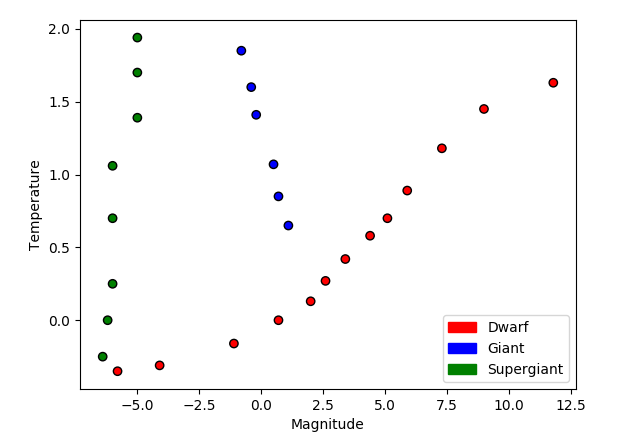
\includegraphics[width=.5\textwidth]{images/star.png}
\end{center}

Please implement the following classifiers in the \verb|SoftmaxRegression| and \verb|KNNClassifier| classes:

\begin{enumerate}[label=\alph*)]

\item \textbf{A multi-class logistic regression classifier} using the softmax activation function, which you investigated in Problem 2. In your implementation of gradient descent, \textbf{make sure to include a bias term and use L2 regularization} with regularization parameter $\lambda = 0.001$. Limit the number of iterations of gradient descent to 200,000, and set the learning rate to be $\eta = 0.001$.

\item \textbf{Another multi-class logistic regression classifier} with feature map $\phi(\boldx) = [\ln (x_1 + 10), x_2^2]^\top$, where $x_1$ and $x_2$ represent the values for magnitude and temperature, respectively.

\item \textbf{A kNN classifier} in which you classify based on the $k = 1$ and $k = 5$ nearest neighbors and the following distance function: $$dist(star_1, star_2) = (mag_1 - mag_2)^2/9 + (temp_1 - temp_2)^2$$
where nearest neighbors are those with the smallest distances from a given point.

  Note 1: When there are more than two labels, no label may have the
  majority of neighbors.  Use the label that has the most votes among
  the neighbors as the choice of label. 

  Note 2: The grid of points for which you are making predictions
  should be interpreted as our test space.  Thus, it is not necessary
  to make a test point that happens to be on top of a training point
  ignore itself when selecting neighbors.

\end{enumerate}

After implementing the above classifiers, complete the following exercises:

\begin{enumerate}
    \item Plot the decision boundaries generated by each classifier for the dataset. Include them in your PDF. 
    Identify the similarities and differences among the classifiers. What explains the differences---in particular, which aspects or properties of each model dictate the shape of its decision boundary? 
    
    \item 
    
    Consider a star with Magnitude 3 and Temperature -2. To which class does each classifier assign this star? Report the classification probabilities of this star for each model. 
    
    Interpret how each model makes its classification decision. What are the pros and cons of each interpretation? What else should we, the modelers, be aware of when making predictions on a test point ``far" from our training data? \textbf{Your response should no be longer than 5 sentences.}
\end{enumerate}
\end{problem}

\newpage
\begin{ans}
    \item Here are the decision boundaries for each plot:
    \newline
    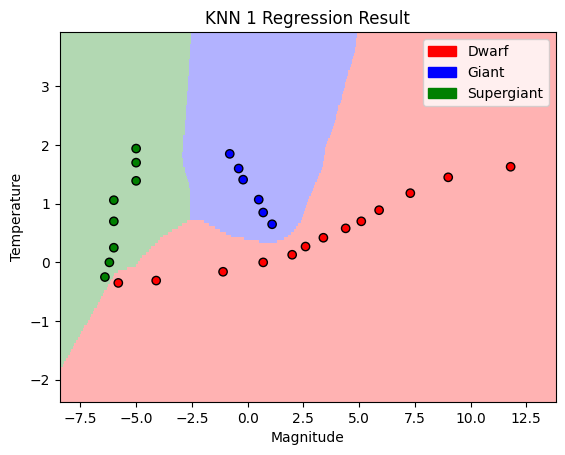
\includegraphics[scale=0.5]{hw2/knn1.png}
    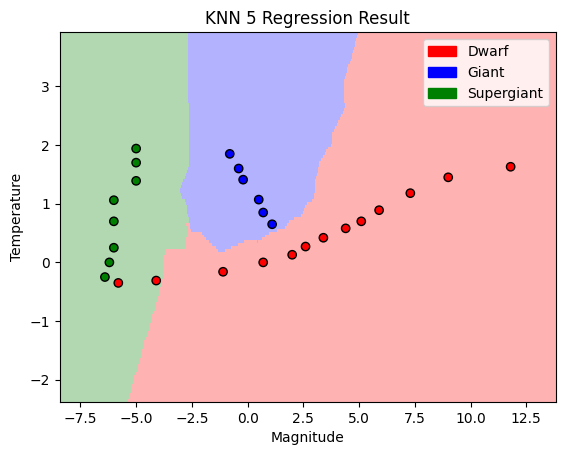
\includegraphics[scale=0.5]{hw2/knn5.png}
    \newline
    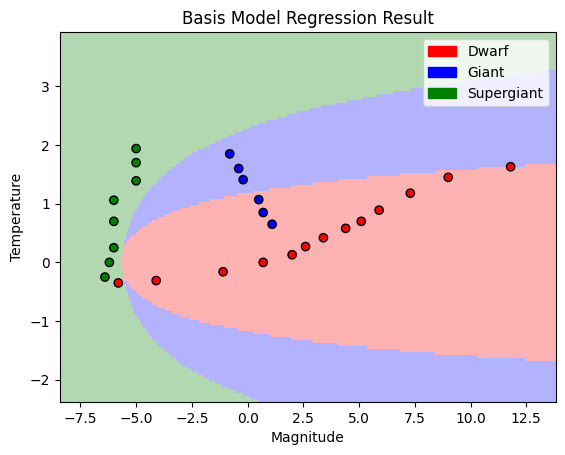
\includegraphics[scale=0.5]{hw2/phi.png}
    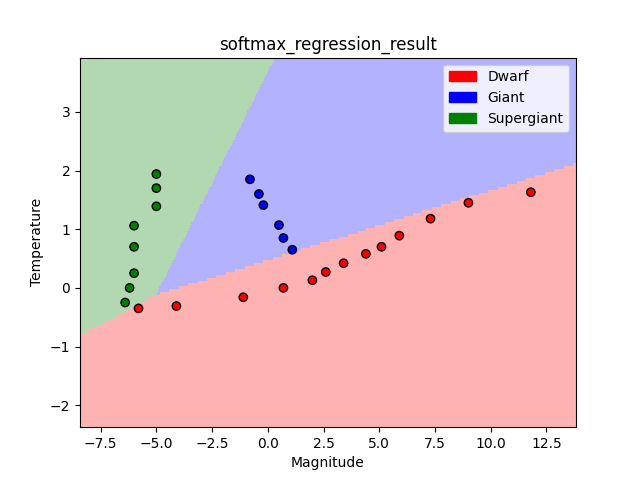
\includegraphics[scale=0.5]{hw2/softmax_regression_result.png}
    \item These graphs make sense because, looking at each graph, 
    \begin{enumerate}
        \item the KNNs form around the closest colors, which is how they work, by definition. KNN-1 has the most intuitive boundaries because it is only looking at the closest point, so it will be the most fit (perhaps overfit) to the data
        \item The Basis model makes sense because the decision boundaries have curves more similar to a log or quadratic function. The regressor was linear, so it could not remove these curves; thus, they carry over to the final graph. 
        \item The Softmax model has linear boundaries, which makes sense because it is simply applying constants to both factors; i.e., it will output linear decision boundaries. 
    \end{enumerate}
    \item The model that doesn't classify this as a dwarf is the basis model, which classifies it as a giant. The softmax model classifies it as such with probability of approximately 1; 
    the basis model classifies it with probability of approximately $99\%$
    Finally, probabilities aren't applicable for our implementation of KNN, since it uses the number of "votes" for each, and picks the majority winner.
    The softmax regressors make their classification decisions by creating a function of the inputs that outputs a real number with how much it gets activated from the features toward being in a certain category, and converting these activations to probabilities with softmax. The KNN models use the $k$-nearest stars--i.e., predict based on stars with similar inputs whose outputs it already knows. Therefore, for the softmax model, the decision boundaries will be extrapolated far outside their useful range; indeed, it's not too likely that these decision boundaries will always be linear, even though that is how they are modelled. For the KNN, too, it will compare to the most similar stars; if these stars are far away from the input, they really aren't that similar, but the model will classify as such, and so will do so with a smaller probability of being right. 
\end{ans}
%%%%%%%%%%%%%%%%%%%%%%%%%%%%%%%%%%%%%%%%%%%%%
% Problem 4
%%%%%%%%%%%%%%%%%%%%%%%%%%%%%%%%%%%%%%%%%%%%%

\begin{problem}[Impact Question: Understanding model-assisted decision making, uncertainty in classification and model interpretation in a high-stakes situation]

\textbf{Prompt:} A pharmaceutical drug company is conducting a clinical drug trial for a devastating disease for which conventional treatment is often ineffective. They want to estimate the effectiveness of a new drug on patients in order to obtain FDA approval and release the drug to the market. They approach you with the results of their clinical trial conducted on 100 patients with features and labels as follows:

Features = \{\textit{age, sex, height, blood pressure, drug administered?}\} \\
Label = \{\textit{Did the patient get cured?}\}

Since testing on a larger patient population is expensive for various reasons, they are interested in developing a machine learning model that will estimate the effectiveness of the drug. They provide you with covariate values of a single unseen patient for testing model performance. 

\begin{enumerate}
    \item You fit a logistic regression model on the 100 observations from the clinical trial and obtain the following coefficients which minimize the negative log likelihood. Let us call this model A:

    $p(y=1 | \mathbf{x}) = \sigma(0.2 + 0.8 *\text{\textit{drug administered?}} - 0.012 *\text{\textit{age}} + 0.45*\text{\textit{sex}} +  0.001*\text{\textit{height}} - 0.007*\text{\textit{blood pressure}})$

    Say you have a female (coded as 0) patient who is age 50, 168cm tall, blood pressure 140. What is the change in classification probability of the patient getting cured when they are administered the drug versus not (please show your work)?  Use your answer to formulate an interpretation of the value of $w_1$ -- the coefficient for \textit{drug administered?} -- for stakeholders in the drug company. The drug company wants you to answer whether or not you see evidence for the efficacy of their drug -- what would you say?

    \item The drug company wants to know you how confident you are that you have the right model, so you decide to sample the existing dataset with replacement to train 100 bootstrapped models. Upon testing these 100 models on the unseen patient, you find that the predictive interval of the classification probability is around $\pm 0.35$ averaged over the bootstrapped models. The drug company is concerned and asks you to check if you can choose alternative models that are more confident in their predictions:
    \begin{enumerate}
        \item You first try adding some interaction terms and train this new model B on the original dataset:

        $p(y=1 | \mathbf{x}) = \sigma(-2 + 5*\text{\textit{drug administered?}} + 2*\text{\textit{age}} - 3.3*\text{\textit{sex}} + 0.001*\text{\textit{height}} + 0.2*\text{\textit{blood pressure}} - 0.12*\text{\textit{age}}*\text{\textit{sex}} -0.34*\text{\textit{height}}*\text{\textit{sex}})$

        Bootstrapping model B 100 times gives you a new predictive interval of $\pm 0.1$ (averaged over bootstrapped models). Why might this be happening -- how would you explain this reduction in uncertainty in model B?

        \item Encouraged by the success of adding interaction terms, you add all possible combinations of interaction terms, repeat the exercise of bootstrapping 100 times and call this model C. This gives you a predictive interval of $\pm 0.39$ averaged over the bootstrapped models. Why might this be happening -- what is the source of this rise in uncertainty? What is a solution to reduce this comparatively large uncertainty, if you wished to keep all the new terms? 
        
        \item Which model (B or C, assuming you can reduce the predictive interval for model C) would you recommend to the drug company and why?
        
    \end{enumerate}

    \item Assume that the drug company has picked model B as their final model of choice because it seems the most confident in its predictions.
    \begin{enumerate}
        \item Suppose that the confidence interval of your estimate of $w_1$ ( coefficient for $drug$ $administered?$) is $\pm 6$. What would you recommend to a critically ill patient who is desperately seeking access to this new (and very expensive, not-covered-by-insurance) drug and why?
        \item The drug company has strong reasons to believe that the drug is indeed effective. What can the drug company do during the clinical trial to tighten the confidence interval of $w_1$?
    \end{enumerate}

\end{enumerate}
\end{problem}

\begin{framed}
\noindent\textbf{Problem 4} (cont.)\\
\begin{enumerate}
\item[3.] (Continued...)
     \begin{enumerate}
     \item[(c)] From prior clinical trials and modeling efforts, the drug company scientists strongly believe that the real value of $w_1$ is either 5 or 1. For now, you take this information as ground truth. In which scenario ($w_1=1$ or $w_1=5$) is it more costly to run the drug trial and demonstrate the effectiveness of the drug? Why?\\
        \textit{Hint:} In which case do you need your confidence intervals for the estimates of $w_1$ to be tighter, to demonstrate drug effectiveness?
        \item[(d)] How do you think we should make use of domain knowledge provided by our partners -- that the real value of $w_1$ is either 5 or 1 -- during model building? For example, would it be a good idea for us to simply fix the parameter $w_1$ to be 5 or 1?
    \end{enumerate}
\item[4.] Let us revisit the data collection process during the clinical trial and consider data collected from two recruitment protocols. In the first recruitment protocol, the drug company publicly advertised the development of this drug to a hospital, encouraging interested patients to sign up for the trial. Among an audience of 100, 50 patients agreed to be administered the drug and 50 choose to opt out and are observed in the study without administering the drug. In the second recruitment protocol, the company was referred 100 patients who have the disease and administered the drug to each patient randomly based on a coin flip. When you train model B on the first dataset, it has a high value of $w_1$ and a small confidence interval of this estimate. In contrast, when you train model B on the second dataset, you get a smaller value for $w_1$ with an equally small confidence interval. Which model would you trust to predict the probability of being cured from the disease given a randomly selected new patient from a Boston hospital? Why?
\textit{Hint:} What confounding factor might we have here?

\end{enumerate}
\end{framed}

\newpage
\begin{ans}
    \item We can solve this by plugging in for the indicator "drug administered" as true and false. However, I will first calculate the rest of the equation to save on repeated computations, saving it as constant $R$ (for rest of the equation)
    $$
    R = 0.2 - 0.012 *50 + 0.45*0 +  0.001*168 - 0.007*140 = -1.212
    $$
    \begin{enumerate}
        \item Suppose the drug is administered. Then we have
        $$
        p(y=1 | \mathbf{x}) = \sigma(R + 0.8 *\text{\textit{drug administered?}}) = \sigma(-0.412)
        $$
        \item Otherwise, we have 
        $$
        p(y=1 | \mathbf{x}) = \sigma(R + 0.8 *\text{\textit{drug administered?}}) = \sigma(R) = \sigma(-1.212)
        $$
    \end{enumerate}
    For our sigmoids, the dependent variable is whether we administer the drug, so we plug into the sum for those two activations as follows:
    $$
    p(y = 1 | \mathbf x, \text{administered drug}) = \frac{e^{-0.412}}{e^{-0.412} + 1} \approx 39.843%
    $$
    $$
    p(y = 1 | \mathbf x, \text{did not administer drug}) = \frac{e^{-1.212}}{e^{-0.412} + e^{-1.212}} \approx 22.934\dots %
    $$
    Informally, I do see a very small amount of evidence for the effectiveness of this drug--40\% is a lot more than 23\%! However, I certainly wouldn't be comfortable releasing the drug to market on this evidence--100 people is a very small sample size, we don't know what the variance in the model is (so I can't perform a t-test or anything like that), and we don't know what the model looks like. As always, in data science, it is crucial to visualize the data. We could have a lack of data in some crucial aspect of this person (for example, some diseases are generally ethnicity-specific, and this model might not account for that). Overall, I would say the results look promising, but we need more data on the trial and possibly more trials. 
    \item 
    \begin{enumerate}
        \item This looks to be a case where the model has more data/more bases, so it can fit the data better. However, it's unclear whether this fit is fitting to the underlying pattern in the data or to noise in the data. 
        \item This looks to be the curse of dimensionality at play: there are too many terms, so the volume of feature space increases exponentially. This harms the model calculating its gradient. Indeed, consider that this leaves us with 31 dimensions = $\sum_{j = 1}^5 5 \choose j$ for an original dataset of $n = 100$. To fix this, we can decrease the number of dimensions and add in a regularization term. We simply don't have enough data to effectively fit this data in 31-dimensional space. Regularization terms help keep the data from overfitting. We can also reduce dimensionality and keep only the most important aspects of these features using, for example, PCA or t-SNE. 
        \item I would recommend Model B, because, as discussed above, model C poorly fit, fitting to the noise because the high dimensionality prevents it from "discerning" patterns in the data. 
    \end{enumerate}
    \item
    \begin{enumerate}
        \item I would allow this patient to access this drug, based on the information I have about it. This depends on what the risks are of this drug and how much more effective it so far has proved to be than the conventional treatments. Overall, however, we should assume that this patient has considered all options and leans toward this new drug. So far, we have promising evidence, and based on the problem formulation, the expected value for them seems to be positive, so it seems like a reasonable decision. In addition, assuming this predictive interval is modeling the distribution as some symmetric, bell-curve-shaped distribution and assuming this model captures the effectiveness of the drug reasonably well, the probability that this drug will prevent the patient from getting better is quite small, since the normal is centered around 5, and the probability that such a normal with $\sigma \approx 3$ takes on a negative value (which will create a worse prediction) is quite low. 
        \item The best thing the drug company can do is increase its sample size - this will decrease the sample's standard deviation. It could also reduce down to the most important factors to mitigate high dimensionality, while adding in other relevant demographic factors. 
        \item In the scenario that $w_1 = 1$: we need far fewer samples for the standard error's interval to exclude negativer values (which, assuming ground truth, means the drug is effective) in the case that $w_1 = 5$ than we do in the case that $w_1 = 1$
        \item This would be a good idea because it could help avoid confounding other factors with the drug's effectiveness, and thus help us create a more accurately-fit model with a tighter interval. 
    \end{enumerate}
    \item I would trust the second model more; in the first model, we likely have an element of self-selection. Perhaps, for example, people trying the new drug are affected with a strain of the disease that causes worse symptoms, but toward which the drug is more effective. 
    
\end{ans}
\newpage
%%%%%%%%%%%%%%%%%%%%%%%%%%%%%%%%%%%%%%%%%%%%%
% Name and Calibration
%%%%%%%%%%%%%%%%%%%%%%%%%%%%%%%%%%%%%%%%%%%%%
\subsection*{Name} John Boesen

\subsection*{Collaborators and Resources}
Whom did you work with, and did you use any resources beyond cs181-textbook and your notes
\newline
 - Collaborators: Minh Le

\subsection*{Calibration}
Approximately how long did this homework take you to complete (in hours)?

12.5

\end{document}
